% !TeX root = ../../main.tex
\resizebox{\textwidth}{\textwidth}{
    \tikzsetnextfilename{source_image}
    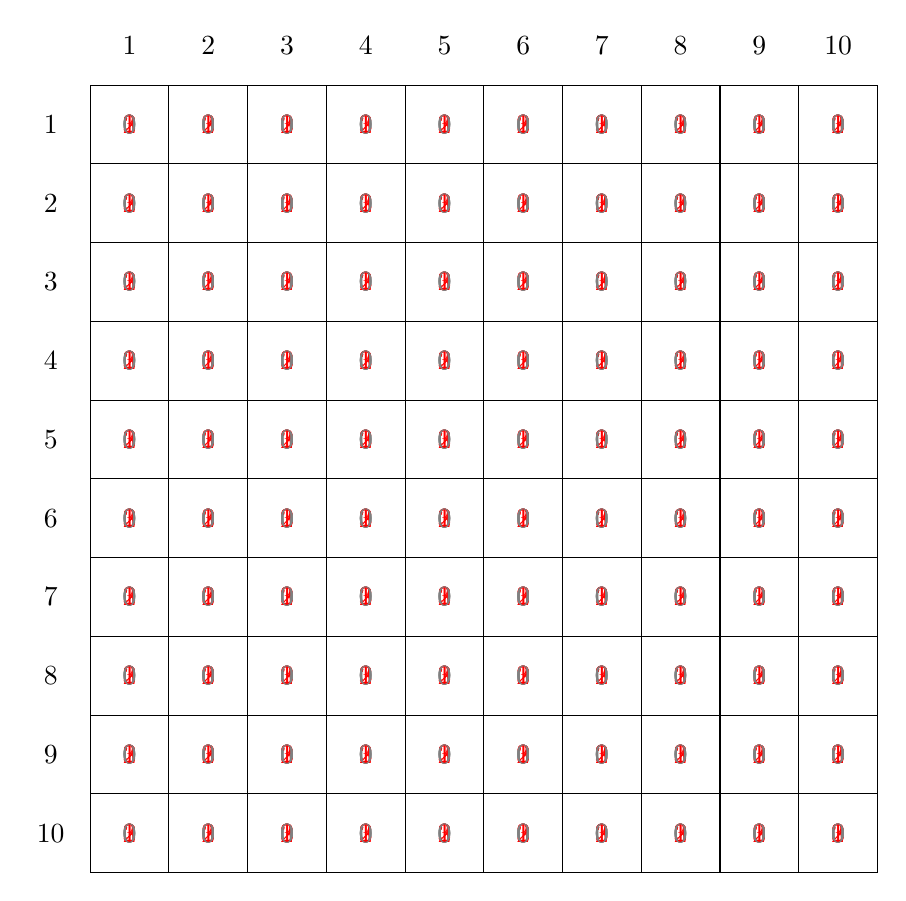
\begin{tikzpicture}
    \foreach \x in {1,...,10} {
        \draw (\x + 0.5, 11.5) node {\x};
    }
    \foreach \y in {10,...,1} {
        \draw (0.5, 11.5 - \y) node {\y};
    }
    \foreach \x in {1,...,10} {
        \foreach \y in {1,...,10} {
            \draw (\x, \y) rectangle (\x +1, \y +1);
            \ifnumequal{\x}{5}{
                \ifnumequal{\y}{5}{
                    \draw[color=red] (\x +0.5, \y +0.5) node {3};
                }{
                    \ifnumequal{\y}{3}{
                        \draw[color=red] (\x +0.5, \y +0.5) node {2};
                    }{
                        \draw[color=gray] (\x +0.5, \y +0.5) node {0};
                    }
                }
            }{
                \ifnumequal{\x}{2}{
                    \ifnumequal{\y}{2}{
                        \draw[color=red] (\x +0.5, \y +0.5) node {1};
                    }{
                        \draw[color=gray] (\x +0.5, \y +0.5) node {0};
                    }
                }{
                    \ifnumequal{\x}{3}{
                        \ifnumequal{\y}{7}{
                            \draw[color=red] (\x +0.5, \y +0.5) node {2};
                        }{                    
                            \draw[color=gray] (\x +0.5, \y +0.5) node {0};
                        }
                    }{
                        \draw[color=gray] (\x +0.5, \y +0.5) node {0};
                    }
                }
            }
        }
    }
    \end{tikzpicture}
}